
\chapter{History}
This chapter summarizes the history of connectionist models used for graph processing. All these models originate from the common feed-forward neural networks (FNNs). The history of neural networks begins in 1943 with the McCulloch–Pitts (MCP) neuron model, following with the Rosenblatt perceptron classifier in 1957. During the following three decades, the feed-forward neural network model was developed and until 1988 a conclusive state was reached in all major fields of related research. The FNN model reached maturity in its field of application: classification and regression performed on unstructured positional samples of fixed size. In the '80s a new branch of the neural networks family began to develop - the recurrent neural networks (RNN). The RNN model is capable of processing sequences of varying length (potentially infinite), which makes them suitable for dealing with time-varying sequences or biological samples of various length~\cite{saha2006prediction}. However, one more approach had to be tried before the RNN model was adapted to processing graph data.

\section{Hopfield networks}
One of the earliest attempts to classify structured data with neural networks was using the Hopfield networks~\cite{goulon2005hopfield}. A common application of a Hopfield is an auto-associative memory, which learns to reproduce patterns provided as its inputs (the learned task is $x_i \Rightarrow x_i$, where $x_i$ is a pattern of fixed size $\forall_{i \in [1..N]} |x_i| = n$). Afterwards, when a new sample is presented to the trained network, the network associates it with the most similar pattern it had learned. However, it was discovered, that by using the Hopfield network to reproduce a predefined successor of a pattern instead of the pattern itself, the network can be used as an hetero-associative memory, capable of reproducing sequences of patterns ($x_i \Rightarrow x_{i+1}$). The next step towards graph processing was to use Hopfield networks to learn the task of reproducing \emph{all} the successors (or predecessors) of a node, that is learn the task $x_i \Rightarrow succ[x_i]$, where $succ[x_i]$ are the successors of node $x_i$ and $\forall_i |succ[x_i]| \leq m \cdot |x_i|$, where $m$ is the maximum outdegree of a node in the analyzed graphs. $NIL$ patterns are used as extra successors whenever a considered node $x_i$ has an outdegree smaller than $m$. The last and somehow different application of Hopfield networks was to use a Hopfield network once again as an auto-associative memory, used for retrieving whole graphs. In such case the graph adjacency matrices ($N \times N$) are encoded into a network having $N(N - 1)/2$ neurons~\cite{goulon2005hopfield}. To obtain an adequate generalisation graphs isomorphic to the training set are generated and fed to the network~\cite{kree1988recognition}.

\section{RAAM}
The Recursive Auto-Associative Memory (RAAM) was introduced by Pollack in 1990~\cite{pollack1990recursive}. The RAAM model is a generalisation of the Hopfield network model~\cite{goulon2005hopfield}, providing means to meaningfully encode directed positional acyclic graphs (DPAGs). This type of graphs contains in particular undirected trees, however in the case of directed graphs their structure may be more complex, as long as there are no cycles. A distinctive feature of the RAAM model is that is can be used to encode graphs with labeled terminal nodes (leaves in the case of trees) only. That is, no node other than the terminal nodes of a graph may be labelled. No edge labels are permitted. The most straightforward domain of application for the RAAM model is thus natural language processing, where sentences can be decomposed to syntax graphs.\\
\noindent The RAAM model is capable of:
\begin{itemize}
	\item building compressed representation of structured data
	\item building meaningful representation: similar samples are represented in a similar way
	\item constrained generalisation: representing data absent in the training set
\end{itemize}
The RAAM model is composed of two units: \emph{compressor} and \emph{reconstructor}. Together they form a three-layer feed-forward neural network which works as an auto-associative memory. The \emph{compressor} is a fully connected two-layer neural network with $n$ inputs and $m$ output neurons. The number of output neurons, $m$ determines the size of a single encoded node representation. The number of inputs, $n$ must be a multiple of $m$, such that $n = k \cdot m$, where $k$ is the maximum outdegree of a node in the considered graphs. For each terminal node its representation consists of its original label. For each non-terminal node $i$ its representation, $x_i$ is built by feeding the compressor with encoded representation of the $i$th nodes children. To assure that the compressed representation is accurate and lossless, it is fed to the \emph{reconstructor}. The reconstructor is also a fully connected two-layer neural network, however it has $m$ inputs and $n$ output neurons. It is fed with compressed representations of nodes and produces the original data that was fed to the compressor. This procedure is repeated for all non-terminal nodes of a graph, until all encoded representations can be accurately decoded into original data. More precisely, the representation $x_i$ of the $i$th node of the graph is given by Eq.~\ref{eq:raam_representation}, where $f$ denotes the function implemented by the compressor unit, $l_i$ - the label of $i$th node, $x_{ch_j}$ - the $j$th child node of the $i$th node, $k$ - the maximum outdegree of a node in the graph. An example of a graph that can be encoded using the RAAM model is presented in Fig.~\ref{fig:tree_for_raam}.

\begin{equation}
x_i = \left\{
\begin{array}{l l}
	l_i & \quad \text{if $i$ is terminal} \\
	f(x_{ch_1}, .., x_{ch_k}) & \quad \text{otherwise}
\end{array}
\right.
\label{eq:raam_representation}
\end{equation}

\begin{figure}
\begin{center}
	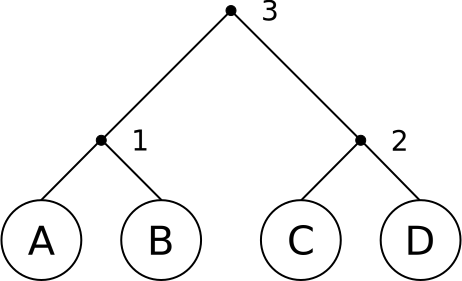
\includegraphics[scale=0.4]{img/tree_for_raam}
	\caption{A sample graph that can be processed using RAAM, only leaves are labelled}
	\label{fig:tree_for_raam}
\end{center}
\end{figure}

To encode the sample graph, first the representations of nodes $1$ and $2$ must be built. The representation of node $1$ is built by feeding the pair of labels $(A, B)$ to the compressor which encodes them into the representation $x_1$. The representation $x_1$ is then fed to the reconstructor, which produces a pair of labels $(A', B')$. If the resulting labels $A'$ and $B'$ are not similar enough to the original labels $A$ and $B$, the error is backpropagated through the compressor-reconstructor three-layer network. Similarly, the pair $(C, D)$ is compressed by the same compressor-reconstructor pair into the representation $x_2$. Then, the pair $(x_1, x_2)$ is once again fed to the compressor, which produces $x_3$, the representation of the root node. This is also the compressed representation of the whole graph, from which the whole graph can be reconstructed by using the reconstructor unit. The training set, consisting of three label pairs, is presented on Fig.~\ref{fig:raam1-3}. The light grey areas denote the compressor network, while the dark grey areas denote the reconstructor. Such a training set (or a larger one if the dataset consists of more than one graph) must be repeatedly processed by the RAAM model in the training phase. When the model is trained, the compression of the whole graph occurs as presented in Fig.~\ref{fig:raam_compression}. Reconstruction of the graph is presented in Fig.~\ref{fig:raam_reconstruction}.

\begin{figure}
\begin{center}
	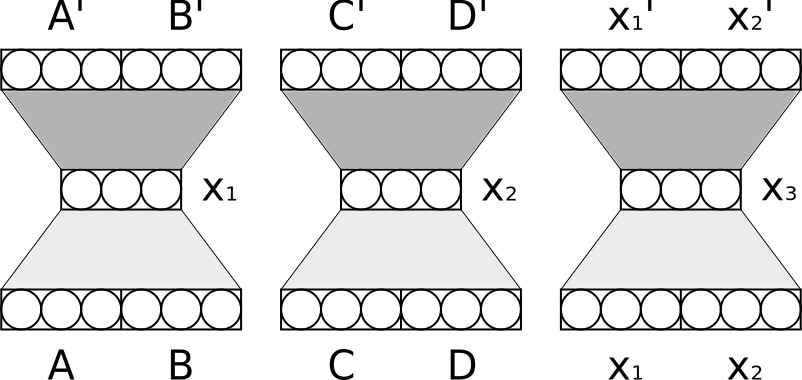
\includegraphics[scale=0.4]{img/raam1-3}
	\caption{Training set for the example graph}
	\label{fig:raam1-3}
\end{center}
\end{figure}

\begin{figure}
\begin{center}
	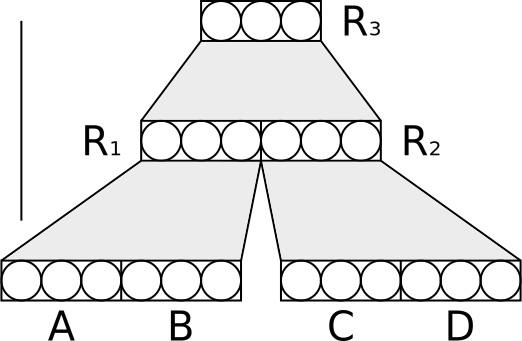
\includegraphics[scale=0.4]{img/raam_encode}
	\caption{Graph compression using trained RAAM model}
	\label{fig:raam_compression}
\end{center}
\end{figure}

\begin{figure}
\begin{center}
	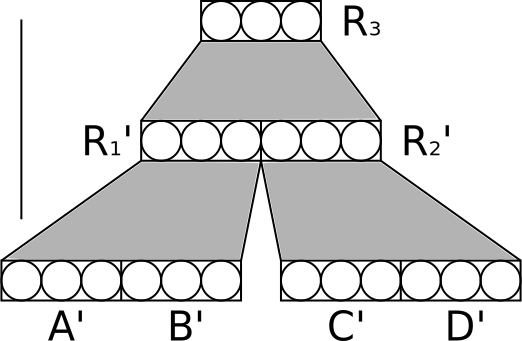
\includegraphics[scale=0.4]{img/raam_decode}
	\caption{Graph reconstruction from $x_3$ using trained RAAM model}
	\label{fig:raam_reconstruction}
\end{center}
\end{figure}



A significant feature of the RAAM model is that a small reconstruction error in the case of non-terminal nodes may render the reconstruction of terminal nodes impossible. Therefore in the process of training a RAAM classifier it is necessary to set the acceptable reconstruction error value much smaller for the non-terminal nodes than for the terminal ones. A major drawback of the RAAM model is the \emph{moving target} problem. That is, a part of the learning set (the representations $x_1$ and $x_2$ from the example) changes during training. In such a case the training phase may not converge to an acceptable state~\cite{goulon2005hopfield}. However, a different training schema is possible, based on recurrent neural networks training procedure~\cite{goulon2005hopfield}. A processing graph is built out of instances of the compressor and reconstructor units (Fig.~\ref{fig:raam_tree}), with structure reflecting the structure of the processed graph (if the dataset consists of multiple graphs, such procedure is repeated for every graph in the dataset). All instances of the compressor unit share their weights and all instances of the reconstructor unit share their weights - which is called the \emph{shared weights} technique. The labels of terminal nodes are fed to the processing network and the resulting error can be backpropagated using the Backpropagation Through Structure~\cite{kuchler1996inductive} algorithm (BPTS). It is worth noting, that the authors of such a modified RAAM model propose using an additional layer of hidden neurons in the compressor and reconstructor units. Such modification allows to partially separate the problem of the data model complexity (i.e. how complex should the RAAM model be to properly compress the data) from the size of terminal node labels which affect the number of inputs to the compressor unit.

\begin{figure}
\begin{center}
	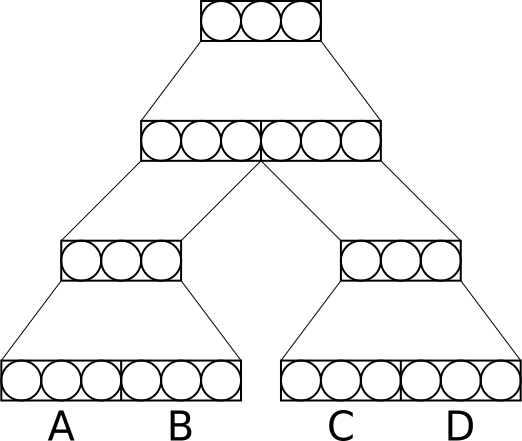
\includegraphics[scale=0.4]{img/raam_tree}
	\caption{Training RAAM using the BPTS procedure}
	\label{fig:raam_tree}
\end{center}
\end{figure}

The most important parameter of the RAAM model is the size of the encoded representation. On one hand, the size should be large enough to contain all the necessary compressed information about the encoded graph. On the other hand, it should be small enough for the compression mechanism to build a minimal representation, which stores only the necessary information about the dataset. If the size is too large, the trained model would store redundant information, memorizing the training set. This would result in a poor ability to process unseen data, which bear resemblance to the training set but is not the same. Experiments with natural language syntax processing~\cite{pollack1990recursive} proved that when the size of the compressed representation is accurate to the problem, the RAAM model is showing some constrained generalisation properties. A drawback of the standard RAAM approach is the termination problem. The model can't distinguish between terminal representations (node labels) and compressed representation which should be further reconstructed. To solve this problem, an additional encoding neuron can be introduced (increasing the representation size by one), which would take a different value for terminal and non-terminal representations~\cite{stolcke1992tree}.

\section{LRAAM}
The most important constraint of the RAAM model is the fact that only terminal nodes of the processed graphs (DPAGs) can contain labels. This problem was addressed by the Labeling RAAM model~\cite{sperduti1994labelling} (LRAAM), which separated the concepts of node labels and node representations. In the RAAM model the terminal nodes are represented by their labels. The LRAAM model introduced the concept of \emph{pointers}, which was used to describe a node representation which has to be learnt, regardless of whether the node is terminal or not. The pointers are produced by compressor units, just like in the case of RAAM and they are decoded into graph structure by reconstructor units. More precisely, the pointer to $i$th node of the graph is calculated according to Eq.~\ref{eq:lraam_pointer}, where $x_i$ stands for pointer to the $i$th node, $f$ is the function implemented by the compressor unit, $l_i$ is the $i$th node label, $x_{ch_j}$ is the $j$th child node of $i$ and $k$ is the maximum outdegree of a node in the considered graph.

\begin{equation}
x_i = f(l_i, x_{ch_1}, .., x_{ch_k})
\label{eq:lraam_pointer}
\end{equation}

Whenever a node outdegree is smaller than $k$ (especially in the case of terminal nodes), the missing child pointers are substituted by the $NIL$ pointer, a special value representing the lack of node. The value of the node label is stacked together with all the pointers values to form an input vector which is fed to the compressor unit. The number of output neurons of the compressor unit (the size of a pointer $x_i$) is $m$. Let's denote the size of the label $l_i$ by $p$. The compressor unit must have $n = p + k \cdot m$ inputs which is also the number of reconstructor unit output neurons.

Just like the RAAM model, the LRAAM model experience the problem of the \emph{moving target}. The same technique of \emph{shared weights} can be applied, which results in building a large recursive neural network composed of identical units. A sample graph is presented in Fig.~\ref{fig:tree_for_lraam}. The recursive network obtained by cloning the compressor and reconstructor units to match the sample graph structure is presented in Fig.~\ref{fig:lraam_tree}. As $A$ and $B$ are terminal nodes, their labels are fed to the compressor unit altogether with $NIL$ pointers representing the missing nodes. Then the compressed representation $x_{A}$ is built for node $A$ and the compressed representation $x_{B}$ is built for node $B$. The representations $x_A$ and $x_B$ are fed altogether with label $C$ to the compressor once again to build the representation $x_C$ of node $C$, which is also the representation of the whole graph.

\begin{figure}
\begin{center}
	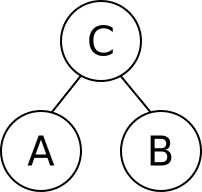
\includegraphics[scale=0.4]{img/tree_for_lraam}
	\caption{A sample graph that can be processed using LRAAM}
	\label{fig:tree_for_lraam}
\end{center}
\end{figure}

\begin{figure}
\begin{center}
	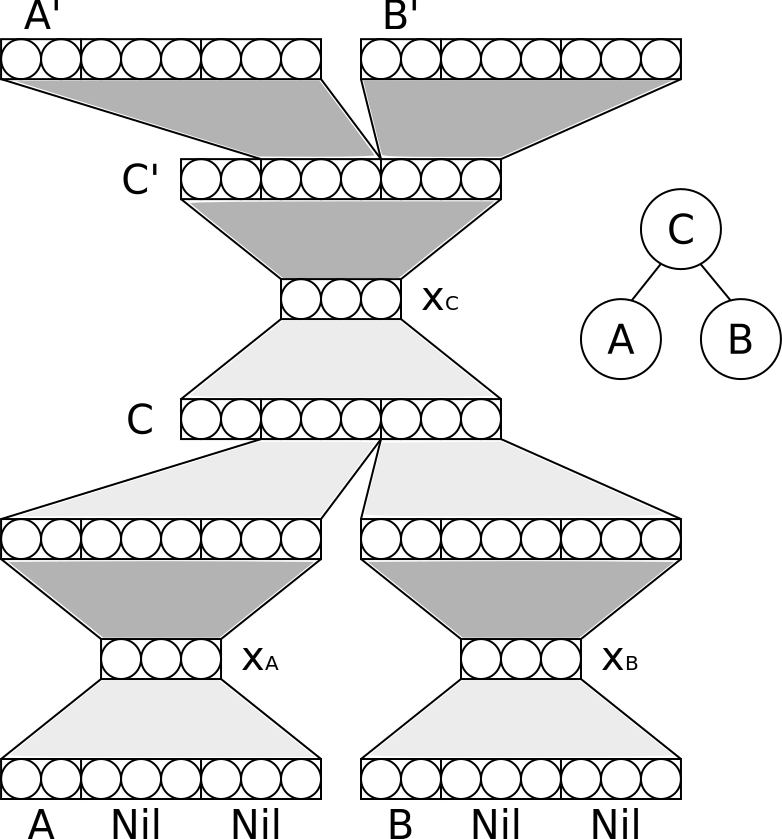
\includegraphics[scale=0.4]{img/lraam_tree}
	\caption{Training LRAAM using the BPTS procedure}
	\label{fig:lraam_tree}
\end{center}
\end{figure}
